\documentclass[danish]{report}

\usepackage[utf8]{inputenc}
\usepackage[danish]{babel}
\usepackage{listings}
\usepackage{color}
\usepackage{courier}
\usepackage{parskip}
\usepackage{graphicx}
\usepackage{mathtools}
\usepackage{amsfonts}

\definecolor{dkgreen}{rgb}{0,0.6,0}
\definecolor{gray}{rgb}{0.5,0.5,0.5}
\definecolor{mauve}{rgb}{0.58,0,0.82}

\lstset{
  frame=,
  language=C,
  aboveskip=3mm,
  belowskip=3mm,
  showstringspaces=false,
  columns=flexible,
  basicstyle={\small\ttfamily},
  numbers=none,
  numberstyle=\tiny\color{gray},
  keywordstyle=\color{blue},
  commentstyle=\color{dkgreen},
  stringstyle=\color{mauve},
  breaklines=true,
  breakatwhitespace=true
  tabsize=4
}

% Title Page
\title{Obligatorisk opgave 2}
\author{Jacob B. Cholewa \& Mathias Pedersen }


\begin{document}
\maketitle
\chapter{Multitrådet sum}
På en multicore processror kan vi kører instruktioner i parallel. Det vil vi i denne opgave udnytte til hurtigere at udregne $ sum = \displaystyle\sum\limits_{i=0}^n \sqrt{i} $.

Først vil vi beskrive hvordan man kører ting i parallel. Vi bruger biblioteket pthread som bruger linux kernes POSIX kald. En tråd har hver sin stack, process nummer, program counter og register, men deler de andre ressourcer i processen med de andre tråde. (se figur \ref{fig:1})


\begin{figure}[H]
\begin{center}
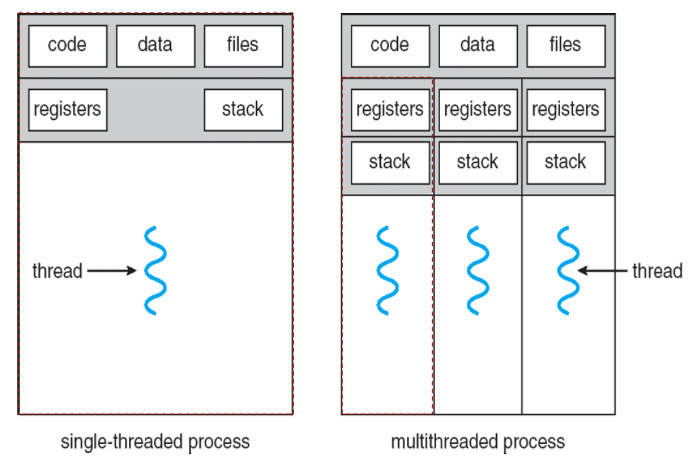
\includegraphics[scale=0.4]{img/1.png}
\caption{Figure der viser enkelt og flertrådede processes}
\label{fig:1}
\end{center}
\end{figure}


Dette gør det nemmere og hurtigere end at oprette en ny process. Hurtigere fordi der ikke skal oprettes lige så meget nyt data og nemmere hvis man har brug for at tilgå den samme data. For at starte en ny tråd kalder vi



\begin{lstlisting}
pthread_create(&tid, NULL, method, args);
\end{lstlisting}

hvor tid er trådens id, NULL bliver sat fordi vi vil køre den med standard indstillinger, method er metoden vi gerne vil køre og args er de argumenter der skal gives til metoden. Metoder der køres skal have typen \textit{void *} og argumentet og parmetre skal også have typen \textit{void *}. Neden for ses den struct vi bruger til at holde input parameteren til vores metode.

\begin{lstlisting}
typedef struct _runnerargs {
        int start;
        int end;
        double *sum;
} Runnerargs;
\end{lstlisting}

For at kunne vente på en tråd bliver færdig, for eksempel hvis vi har brug for et resultat, kan vi bruge 

\begin{lstlisting}
pthread_join(&tid, NULL);
\end{lstlisting}


For at kunne køre udregningen i parallel skal vi kunne opdele beregningen til mindre udregninger. Det kan vi gøre fordi følgende gælder.

\begin{equation*}
sum = \displaystyle\sum\limits_{i=0}^n \sqrt{i} = \sqrt{0} + \displaystyle\sum\limits_{j=0}^{p} \left( \displaystyle\sum\limits_{i=\frac{n}{p}*j+1}^{\frac{n}{p}} \sqrt{i} \right), \frac{n}{p} \in \mathbb{N} \text{ hvor } p \text{ lig antallet af tråde}
\end{equation*}


Vi har implementeret dette med følgende kode stykke.

\begin{lstlisting}
int cut, last = 0, threadsleft = nthreads;
for(int i = 0; i < nthreads; i++){
    /* calculates the range that thread i should calculate */
    cut = sumto / threadsleft;
    /* prepares the argument for thread i */
    args[i] = (Runnerargs)  {(last + 1),(last + cut),&sum[i]};

    /* starts a new thread that runs the method runner with arguments args[i] */
    pthread_create(&tid[i],NULL,runner,&args[i]);

    /* removes the range from the amount still needed to be calculated */
    sumto -= cut;

    /* decrement the amount of threads needed to be started */
    threadsleft--;

    /* saves the last element calculated by this thread */
    last+=cut;
}
\end{lstlisting}

For at undgå at $\frac{n}{p}$ skal være et naturligt tal deler vi mængden vi skal udregne med antal tråde der mangler at blive startet og trækker den mængden fra den samlede mængde. På den måde sørger vi altid for at udregne hele mængden selvom den ikke kan deles med antal tråde. 

Til sidst venter vi på at alle trådene er færdige med at beregne og lægger resultaterne sammen.

\begin{lstlisting}    
double total_sum = 0;
for(int i = 0; i < nthreads; i++){
    pthread_join(tid[i],NULL);
    total_sum += sum[i];
}
\end{lstlisting}

Vi har testet det på en computer med fire kerner (se figure \ref{fig:3}) og der ses det tydeligt køretiden forbedres når man kører ligeså mange, eller flere, tråde som computeren har kerner.

\begin{figure}[H]
%\begin{center}
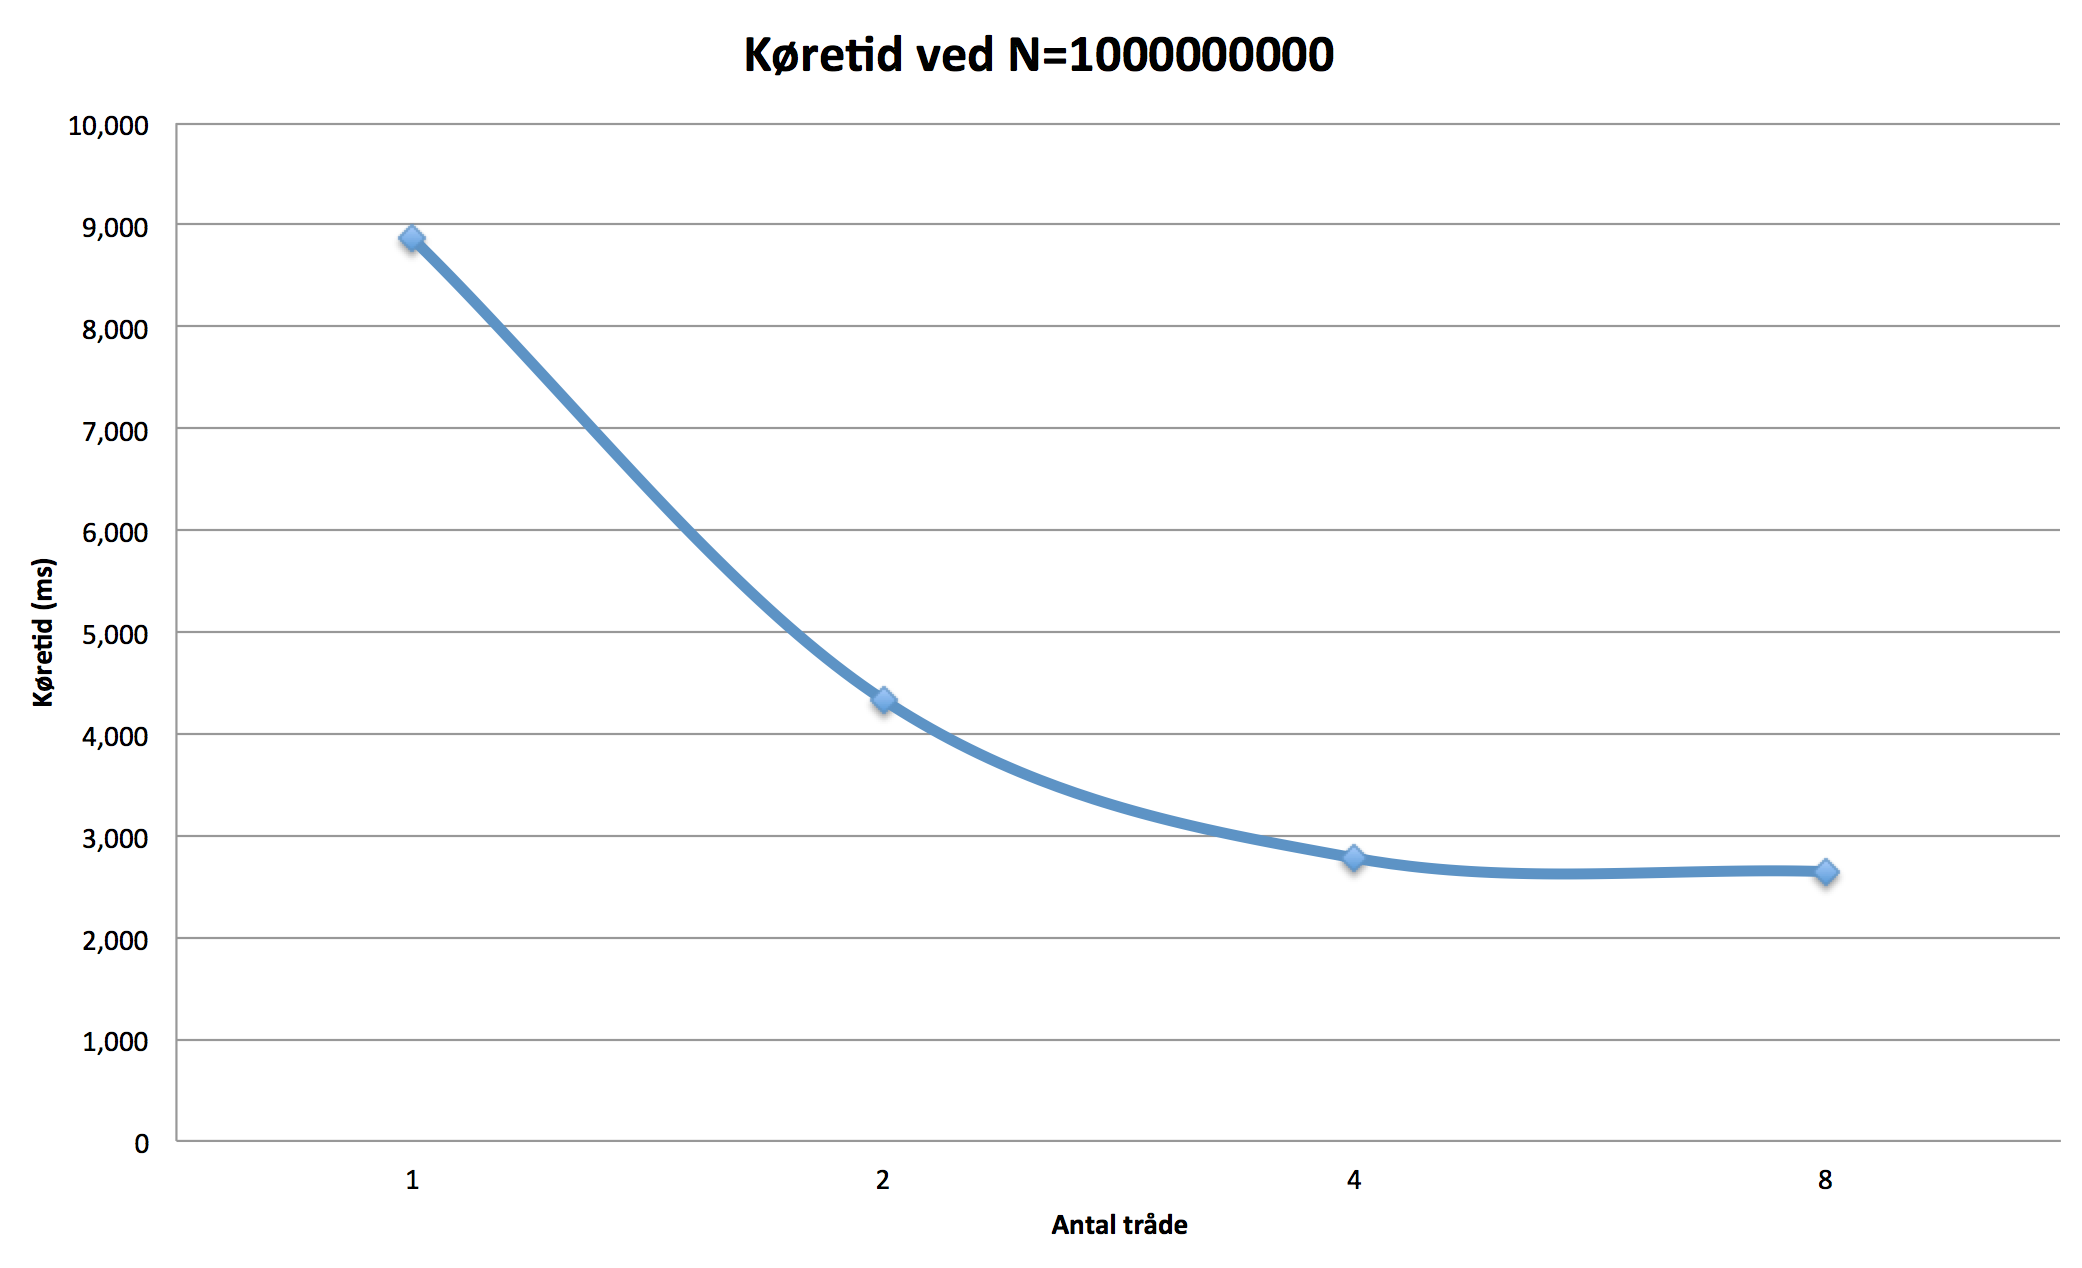
\includegraphics[width=\linewidth]{img/3.png}
\caption{Speed-up graf}
\label{fig:3}
%\end{center}
\end{figure}

\chapter{Multitrådet FIFO buffer som kædet liste}
I denne opgave arbejder vi med implementeringen af en trådsikker kædet liste der i næste opgave vil blive brugt som FIFO buffer.

En kædet liste består af elementer der peger på næste element i listen. Den adskiller sig altså fra et array ved ikke at skulle ligge sekventielt i hukommelsen og i det at den ikke har en fast længde(og krævet hukommelse).

Det første skridt er at færdiggøre implementeringen af den givne kode: \textit{list\_add()} og \textit{list\_remove()}. Listen vi vil implementere er en FIFO, First In First Out. Det vil altså sige at når vi indsætter i listen skal det nye element på første plads. Det opnås på følgende måde:

\begin{lstlisting}    
/* list_add: add node n to list l as the last element */
void list_add(List *l, Node *n)
{
	n -> next = l -> first;
	l -> first = n;
	l -> len++;
}
\end{lstlisting}

I remove funktionen tager vi igen første element, fjerner det fra listen og returnere en pointer til elementet. Helt specifikt fjernes elementet fra listen ved først at gemme en pointer til elementet, så at sætte listens første element til det udtaget elements næste, og til sidst tælle længden af listen en ned.

\begin{lstlisting}    
/* list_remove: remove and return the first (non-root) element from list l */
Node *list_remove(List *l)
{
	if(l -> len <= 0) return NULL;

	Node *n = l -> first;
	l -> first = n -> next;
	l -> len--;

	return n;
}
\end{lstlisting}

Det næste skridt i opgaven er at gøre listen trådsikker. Scenariet er at vi har flere tråde der arbejder på samme liste element i hukommelsen. Vi vil gerne sikre at to eller flere tråde ikke kommer i racecondition når de arbejder med de overstående funktioner. En kædet liste er meget skrøbelig da en pointer er livslinjen til at få fat i resten af listen, og hvis flere tråde brugte overstående funktioner kunne det gå galt. Løsningen er at bruge mutex låse.

I vores implementation bruger vi pthread's mutex, som er et objekt vi binder til listen. På den måde har hver liste i hukommelsen et mutex. Mutex'et locker vi i starten af hhv. add og remove funktionerne, og unlocker i slutningen. Koden ind i mellem er altså vores critical section, som afhænger af to ting. Først arbejder vi med værdier som kun en tråd må arbejde på. Derfor bruger vi samme mutex i funktionerne der arbejder med disse variabler. Dernæst vil vi også gerne have at ændringerne i en given critical section sker i træk uden at en anden tråd byder ind i mellem.


\begin{lstlisting}    
pthread_mutex_lock(&l->mutex);
//CRITICAL SECTION
pthread_mutex_unlock(&l->mutex);
\end{lstlisting}

Afslutningsvist, for at teste at dette virker, har vi lavet en stress test: Et program der opretter et givent antal tråde som alle arbejder på samme liste. De tilføjer og fjerner alle 100 elementer konstant. Listen uden mutex crasher hurtigt og den med mutex kører fint.


\chapter{Producer-Consumer med bounded buffer}

I denne opgave implementerer vi et producer-consumer system med fælles buffer i form af listen fra forrige opgave. Systemet skal tage argumenter i form af antallet af producers, antallet af consumers, størrelsen af den delte buffer, samt antallet af produkter der i alt skal produceres.

Ud fra argumenterne vil der blive oprettet et vis antal tråde til producers og consumers. Hver tråd kører hhv. funktionen \textit{producer()} og \textit{consumer()} som ses fuldt implementeret herunder.

Hver tråd kører i et while true loop. Vores krav er at en producer ikke må putte flere produkter i bufferen end den givne størrelse, og at den ikke må producere flere produkter end maximum. En consumer skal vente på at der er noget i listen.

\begin{lstlisting}    
void *producer(void *args){
	int nr = args;
	while(1){
	
		/* Incrementing produced with symaphore psem */
		sem_wait(&psem); //waiting for the given symaphore
		if(++produced > np){ //Incrementing *p and checking if the value is less than the maximum amount of products
			sem_post(&psem); //Releasing the lock before returning
			return 0; //Exiting the producer
		}
		sem_post(&psem); //Adding to the psem symaphore
		
		sem_wait(&empty); //Waiting if the list is full
		Node *n = node_new_str("string");
		list_add(buffer, n);
		printf("Producer %i produced %s. Items in buffer: %i (out of %i)\n",nr,n->elm,buffer->len,buffer_size);
		sem_post(&full); //Adding to the full symaphore
		rsleep(500); //Waiting a for a random range of 0 and 2*500ms
	}
}
\end{lstlisting}

\begin{lstlisting}    
void *consumer(void *args){
	int nr = args;
	while(1){
	
		/* Incrementing consumed with symaphore csem */
		sem_wait(&csem); //waiting for the given symaphore
		if(++consumed > np){ //Incrementing *p and checking if the value is less than the maximum amount of products
			sem_post(&csem); //Releasing the lock before returning
			return 0; //Exiting the consumer
		}
		sem_post(&csem); //Adding to the csem symaphore
		
		sem_wait(&full); //Waiting if list is empty
		Node *n = list_remove(buffer);
		printf("Consumer %i consumed %s. Items in buffer: %i (out of %i)\n",nr,n->elm,buffer->len,buffer_size);
		sem_post(&empty); //Adding to the empty symaphore
		rsleep(500); //Waiting a for a random range of 0 and 2*500ms
	}
}
\end{lstlisting}

For at sikre at kravene bliver overholdt bruges semaforer. Et semafor er et heltal og kan enten bruges som mutex(0 eller 1), eller som tællesemafor. I vores implementation bruges semaforerne som tællere til at overholde disse krav. Vi bruger altså først og fremmest to semaforer: \textit{empty, full}, som initialiseres på følgende måde:

\begin{lstlisting}    
/* Initializing semaphores */
sem_init(&empty, 0, buffer_size);
sem_init(&full, 0, 0);
\end{lstlisting}

Vi bruger semaforerne i to funktioner; sem_wait() og sem_post(). I wait tjekkes semaforet, og hvis det er over 0 trækkes 1 fra, ellers blokeres tråden. I post lægges der 1 til semaforet, og hvis det er lig med 0 låses det op. Produceren waiter altså på empty, som initialiseres med buffer_size, hvilket trækker 1 fra. Det vil sige at hvis empty er 0, vil der ikke blive produceret, da listen er fuld. Hvis produceren får lov at producere slutter den med at poste på semaforet full hvilket vil tælle den en op, og evt. vække consumer tråde der venter på produkter. Consumeren venter på full der beskriver antal produkter i bufferen, og slutter med at poste på empty, hvilket tæller den en op, og evt. vækker producere tråde der venter på at måtte producere.

De to sidste semaforer, \textit{csem og psem}, bruger vi som mutexes, for at undgå at der opstår raceconditions når consumed og produced tælles op, da denne operation ikke er atomisk. Vi er nød til at holde styr på hvor mange produkter der er produced og consumed for på rigtig vis at afslutte produktionen ved det givne maximum.


\chapter{Banker’s algorithm til håndtering af deadlock}

Banker's algoritme bruges til at afgøre om der kan opstå deadlocks. Deadlock er et stadie hvor tråd A venter på tråd B og tråd B venter på tråd A der derfor begge vil vente uendeligt. Se figure \ref{fig:2}. Samme problem stilling gælder også for en kæde hvor A venter på B der venter på C der venter på A, altså når der er en cyklus.

Banker's algoritmen kan bruges hvis man på forhånd kender processens maks resurse forbrug og hvis processer når den har alle sine resurser returnerer dem i endelig tid. Ud over det virker den kun for et statisk antal processer.


Algoritmen sørger for at før en process bliver tildelt resurser checker systemet om tildelingen vil kunne føre til en usikker tilstand. Hvis tilstanden er sikker bliver resurserne tildelt, ellers bliver processen tvunget til at vente til at den kan få tildelt resurserne i en sikker tilstand.

Til det har vi en vektor til at holde styr på hvor mange resurser der er tilgængelige (available) og tre matriser til at holde styr, for hver process, for mange resurser den maksimalt bruger (max), nuværende har allokeret (allocated) og hvor mange den mangler for at blive færdig (need).

Da vi gerne dynamisk vil kunne oprette matriserne bruger vi \textit{malloc} 
til at reservere plads på hoben. Neden for ses metoden \textit{alloc\_memory} som vi bruger til at reservere plads til vores matriser. 

\begin{lstlisting}
/* Allocate memory needed for runtime */
void alloc_memory(){
        s = (State *) malloc(2 * sizeof(int *) + 3 * sizeof(int **));
        s -> resource   =       malloc(n* sizeof(int));
        s -> available  =       malloc(n * sizeof(int));
        s -> max        =       malloc(m * sizeof(int *));
        s -> need       =       malloc(m * sizeof(int *));
        s -> allocation =       malloc(m * sizeof(int *));

        work            =       malloc(n * sizeof(int));
        finish          =       malloc(m * sizeof(int));

        for(int i = 0; i < m; i++){
                s -> max[i] = malloc(n * sizeof(int));
                s -> need[i] = malloc(n * sizeof(int));
                s -> allocation[i] = malloc(n * sizeof(int));
        }
}
\end{lstlisting}

På samme måde bruger vi \textit{free\_memory} metoden  til at frigive pladsen igen når vi er færdige med den.
\begin{lstlisting}
/* free memory allocation during runtime */
void free_memory(){
        for(int i = 0; i < m; i++){
                free(s -> max[i]);
                free(s -> need[i]);
                free(s -> allocation[i]);
        }
        free(s -> max);
        free(s -> need);
        free(s -> allocation);
        free(s -> available);
        free(s -> resource);
        free(finish);
        free(work);
        free(s);
}
\end{lstlisting}

Når vi har allokeret vektorerne og matriserne og defineret nogle processer, resurser og deres tilhørende værdier kan vi tjekke om de til at starte med er i en sikker tilstand. Det gør vi med følgende kode.

\begin{lstlisting}
/* Bankers safty algorithm */
int safety_check(){
        /* Set work = available */
        for(int i = 0; i < n; i++){
                work[i] = s->available[i];
        }

        /* set Finish[i] = false for all i */
        for(int i = 0; i < m; i++){
                finish[i] = 0;
        }

        /* If finish[i] == false and need[i] <= work then allocate, set finish[i] to true and restart loop */
        for(int i = 0; i < m; i++){
                if(finish[i] == 0 && slarger(s->need[i], work, n)){
                        addarr(work, s->allocation[i], n);
                        finish[i] = 1;
                        i = 0;
                }
        }

        /* if any element in finish == false return 0, else return 1  */
        for(int i = 0; i < m; i++){
                if(finish[i] == 0) return 0;
        }
        return 1;
}
\end{lstlisting}


Når en process requester resurser tildeler vi resurserne, tjekker om det ender i en sikker tilstand, og hvis ikke får vi den til at vente til en sikker tilstand opstår.

\begin{lstlisting}
/* Allocate resources in request for process i, only if it
   results in a safe state and return 1, else return 0 */
int resource_request(int i, int *request)
{
        //Checking if the request exceeds the max need
        if(!slarger(request, s->need[i], n)){
                printf("ERROR!\n");
                exit(1);
        }

        /* Aquire lock for state */
        pthread_mutex_lock(&state_mutex);

        /* if request > avalible then return 0*/
        if(!slarger(request, s->available, n)){
                pthread_mutex_unlock(&state_mutex);
                return 0;
        }

        /* Allocate resources */
        subarr(s->available, request, n);
        addarr(s->allocation[i], request, n);
        subarr(s->need[i], request, n);

        /* Check if safe state else reverse allocation and return 0 */
        if(!safety_check()){
                addarr(s->available, request, n);
                subarr(s->allocation[i], request, n);
                addarr(s->need[i], request, n);
                pthread_mutex_unlock(&state_mutex);
                return 0;
        }

        /* Release lock for state */
        pthread_mutex_unlock(&state_mutex);
        return 1;
}
\end{lstlisting}

På denne måde kan vi sikre at en proces kun bliver tildelt resurser hvis det resulterer i en sikker tilstand.

Gennem vores tests fandt vi et problem med den allerede implementerede metode \textit{generate\_release} og problemet ligger i den måde det frigiver ressourcer på

\begin{lstlisting}
/* Generate a release vector */
void generate_release(int i, int *request)
{
        int j, sum = 0;
        while (!sum) {
                for (j = 0;j < n; j++) {
                        request[j] = s->allocation[i][j] * ((double)rand())/ (double)RAND_MAX;
                        sum += request[j];
                }
        }
        printf("Process %d: Releasing resources.\n",i);
}
\end{lstlisting}

Denne metode terminer kun hvis request vektoren bliver allokeret forskelligt fra $[0,0,0]$, men hvis allocation veltoren er $[0,0,1]$ eller en anden kombination af de to tal er det meget usandsynligt at metoden teminerer. \textit{((double)rand())/ (double)RAND\_MAX} returnere et tal mellem $0$ og $1$, men da allocation vektoren er $[0,0,1]$ vil sum kun overstige $0$ hvis det tilfældige tal er \textit{RAND\_MAX} da tallet ellers vil blive nedrundet til $0$ hvilket gør at metoden aldrig (usandsynligt) terminer. Samme problem gælder for \textit{generate\_request} metoden hvis need vektoren indeholder kun $0$ og $1$.


\begin{figure}[H]
\begin{center}
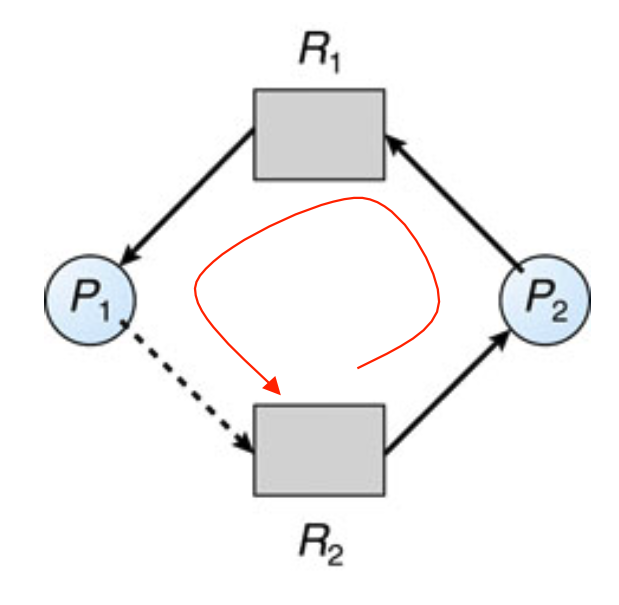
\includegraphics[scale=0.4]{img/2.png}
\caption{Figure der viser en deadlock}
\label{fig:2}
\end{center}
\end{figure}


\end{document}          
